\section*{ÔN TẬP CHƯƠNG II}
\subsection{CÂU TRẮC NGHIỆM NHIỀU PHƯƠNG ÁN LỰA CHỌN}
\textit{Thí sinh trả lời từ câu 1 đến câu 18. Mỗi câu hỏi thí sinh chọn một phương án.}
\Opensolutionfile{ans}[ans/G12Y24B15TN]
% ===================================================================
\begin{ex}
Đường biểu diễn sự biến thiên của áp suất theo thể tích của một lượng khí lí tưởng nhất định ở hình vẽ bên mô tả quá trình nào?
\begin{center}
	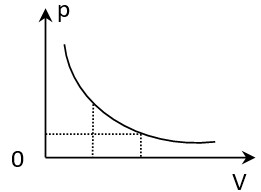
\includegraphics[width=0.35\linewidth]{../figs/VN12-Y24-PH-SYL-016-1}
\end{center}	
	\choice
	{Đẳng tích.}
	{Đẳng entropy.}
	{Đẳng áp.}
	{\True Đẳng nhiệt.}
	\loigiai{}
\end{ex}
% ===================================================================
\begin{ex}
	Đại lượng nào sau đây \textbf{không phải} là thông số trạng thái của một lượng khí?
	
	\choice
	{Thể tích.}
	{Áp suất.}
	{\True Khối lượng.}
	{Nhiệt độ.}
	\loigiai{}
\end{ex}
% ===================================================================
\begin{ex}
	Với $\Delta U$, $Q$, $A$ lần lượt là độ biến thiên nội năng hệ, nhiệt lượng và công hệ nhận thì công thức đúng của định luật I nhiệt động lực học là
	\choice
	{$\Delta U=A$.}
	{$\Delta U=Q$.}
	{$\Delta U=Q\cdot A$.}
	{\True $\Delta U=Q+A$.}
	\loigiai{}
\end{ex}
% ===================================================================
\begin{ex}
Phát biểu nào sau đây là đúng với nội dung định luật Boyle?	
	\choice
	{\True Trong quá trình đẳng nhiệt của một lượng khí nhất định, áp suất tỉ lệ nghịch với thể tích.}
	{Trong quá trình đẳng áp của một khối lượng khí xác định, áp suất và thể tích là một hằng số.}
	{Trong quá trình đẳng tích của một khối khí xác định, tích của áp suất và thể tích là một hằng số.}
	{Trong quá trình đẳng nhiệt của một lượng khí nhất định, áp suất tỉ lệ thuận với thể tích.}
	\loigiai{}
\end{ex}
% ===================================================================
\begin{ex}
	Hiện nay, nhiệt độ thấp nhất trong phòng thí nghiệm mà con người thực hiện được vào khoảng
	
	\choice
	{$\SI{-9}{\kelvin}$.}
	{$\SI{-9}{\celsius}$.}
	{\True $\SI{E-9}{\kelvin}$.}
	{$\SI{E9}{\kelvin}$.}
	\loigiai{}
\end{ex}
% ===================================================================
\begin{ex}
Điều nào sau đây là \textbf{sai} khi nói về mô hình động học phân tử chất khí?
	
	\choice
	{Chất khí được cấu tạo từ các nguyên tử, phân tử riêng biệt.}
	{Các phân tử chuyển động hỗn loạn, không ngừng.}
	{Các nguyên tử, phân tử tương tác với nhau bằng lực hút và lực đẩy.}
	{\True Các phân tử luôn hút nhau để tạo thành chất.}
	\loigiai{}
\end{ex}
% ===================================================================
\begin{ex}
	Hệ thức nào sau đây phù hợp với định luật Charles?
	\choice
	{$V\sim t$.}
	{\True $\dfrac{V_1}{T_1}=\dfrac{V_2}{T_2}$.}
	{$\dfrac{V}{t}=\text{hằng số}$.}
	{$\dfrac{V_1}{V_2}=\dfrac{T_2}{T_1}$.}
	\loigiai{}
\end{ex}
% ===================================================================
\begin{ex}
	Trong quá trình đẳng tích thì áp suất của một lượng khí xác định
	\choice
	{tỉ lệ thuận với bình phương của nhiệt độ tuyệt đối.}
	{\True tỉ lệ thuận với nhiệt độ tuyệt đối.}
	{tỉ lệ thuận với căn bậc hai của nhiệt độ tuyệt đối.}
	{tỉ lệ nghịch với nhiệt độ.}
	\loigiai{}
\end{ex}
\Closesolutionfile{ans}